\scanpage{65}
\mspage{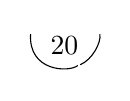
\begin{tikzpicture}[baseline=(n.base)]\node (n) at (0,0) {20};\draw (-.43,.15) .. controls (-.46,-.33) and (.06,-.34) .. (.17,-.25);\draw (.20,-.24) .. controls (.35,-.18) and (.47,.04) .. (.45,.15);\end{tikzpicture}}

Ce sont aussi les \deleted{diagr.} flèches en traits pleins du diagramme fondamental (17)

Avec l'ens ordonné $I$, fabriquons donc un \deleted{ens ordonné} \uline{diagramme} dont les sommets sont \deleted{des ``lettres'' $\unsure{x|i}\ i^*$} des symboles \deleted{$i_{**}$} $[i]$, $[i,j]$, $[i,j]^*$, où $i,j\in I$, $j$ un succ. de $i$. Les flèches du diagramme sont \unsure{des|de} trois types qui sont toutes décrites ds
\diagram{$(19)\qquad$\begin{tikzcd}[column sep=large,row sep=large]
{[i,j]^*} \arrow[r] \arrow[d] & {[i,j]} & i^* \arrow[l] \\
{[j]^*} & &
\end{tikzcd}}

Désignons par $\widetilde I$ ce diagramme, dont l'ens des sommets \deleted{s'identifie} \unsure{à|a} \deleted{$\unsure{I\times I_\Delta}$} \inserted{le cardinal} $\operatorname{card}I+2\nu$ \deleted{\unsure{card.}} \inserted{où $\nu=\operatorname{card}$} de l'ens des drapeaux $(i<j)$ ``élémentaires'' \inserted{i.e. tels que $j$ soit successeur de $i$} et le nb des flèches est $3\nu$. Si $I$ contient \unsure{ex.ctt|ex.ct} deux élts $i,j$ avec $i<j$, \inserted{i.e. $I\simeq\Delta_1$,} ce diagramme est en. (19). Si $I=\Delta_r=(0,1,\ldots,r)$, on trouve (en employant maintenant les symboles pour les $X_i^*,V_{ij}^*,V_{ij}$ qui réalisent le diagramme)

\margin{64}
